% NP-Hardness Part 1 -- Metropolis beamer slides
% Compile: pdflatex np-hardness-part-1.tex (x2)
\documentclass[10pt,aspectratio=169]{beamer}

\usetheme{metropolis}
\metroset{block=fill, numbering=fraction, progressbar=frametitle}

\usepackage[T1]{fontenc}
\usepackage{amsmath, amssymb}
\usepackage{booktabs}
\usepackage{tikz}
\usetikzlibrary{arrows.meta, positioning, calc}

% ---- colors -------------------------------------------------------------
\definecolor{mLightBlue}{HTML}{4C72B0}
\definecolor{mGreen}{HTML}{55A868}
\definecolor{mRed}{HTML}{C44E52}
\definecolor{mGray}{HTML}{BFBFBF}
\definecolor{mOrange}{HTML}{DD8452}
\setbeamercolor{alerted text}{fg=mRed}

% ---- helpers ------------------------------------------------------------
\tikzset{
  vtx/.style={draw, circle, minimum size=6.5mm, inner sep=0pt, font=\small,
              fill=white},
  edg/.style={thick, mGray!80!black},
  cA/.style={vtx, fill=mRed!35},
  cB/.style={vtx, fill=mLightBlue!35},
  cC/.style={vtx, fill=mGreen!40},
  pick/.style={vtx, fill=mOrange!55},
  box/.style={draw, thick, rounded corners=3pt, minimum height=8mm,
              minimum width=18mm, align=center, font=\small},
  arr/.style={thick, -{Stealth[length=2.5mm]}},
  % overlay-aware keys: onslide=<2->{cA}
  onslide/.code args={<#1>#2}{\only<#1>{\pgfkeysalso{#2}}},
}

% The 7-vertex graph used for 3-coloring. Arguments: styles for v1..v7.
\newcommand{\sevengraph}[7]{%
  \node[#1] (v1) at (0,0)        {1};
  \node[#2] (v2) at (0,1.6)      {2};
  \node[#3] (v3) at (1.39,0.8)   {3};
  \node[#4] (v4) at (1.39,-0.8)  {4};
  \node[#5] (v5) at (0,-1.6)     {5};
  \node[#6] (v6) at (-1.39,-0.8) {6};
  \node[#7] (v7) at (-1.39,0.8)  {7};
  \draw[edg] (v2)--(v3)--(v4)--(v5)--(v6)--(v7)--(v2);
  \draw[edg] (v1)--(v2); \draw[edg] (v1)--(v4); \draw[edg] (v1)--(v6);
  \draw[edg] (v3) to[bend right=20] (v6); \draw[edg] (v4) to[bend left=20] (v7);
}

% ---- title --------------------------------------------------------------
\title{NP-Hardness, Part 1}
\subtitle{Decision Problems, P, Reductions, NP}
\date{}
\author{}

\begin{document}

\maketitle

% =========================================================================
\begin{frame}{Easy or Hard?}
  So far: problems with efficient algorithms. Small changes to a problem can
  make it seem far harder.

  \bigskip
  \begin{center}
  \begin{tabular}{ll}
    \toprule
    we know a fast algorithm & no fast algorithm known \\
    \midrule
    shortest simple path & longest simple path \\
    Euler tour (every \alert{edge} once) & Hamiltonian cycle (every
      \alert{vertex} once) \\
    2-coloring a graph & 3-coloring a graph \\
    minimum spanning tree & traveling salesman tour \\
    \bottomrule
  \end{tabular}
  \end{center}

  \pause
  \bigskip
  This part of the course: how to give evidence that a problem is
  \alert{hard}, so we can stop looking for an efficient algorithm.
\end{frame}

% =========================================================================
\section{Decision Problems}

\begin{frame}{Decision Problems}
  \begin{block}{Definition}
    A \alert{decision problem} is a problem whose answer is \textbf{yes} or
    \textbf{no}.
  \end{block}

  Every input is either a \alert{yes-instance} or a \alert{no-instance}.

  \bigskip
  Three running examples:
  \begin{itemize}
    \item \textbf{Independent Set}: given $G$ and $k$, is there a set of
          $\ge k$ vertices with no edge between any two of them?
    \item \textbf{Subset Sum}: given integers $S$ and a target $t$, does some
          subset of $S$ sum to exactly $t$?
    \item \textbf{Graph Coloring}: given $G$ and $k$, can the vertices be
          colored with at most $k$ colors so that adjacent vertices differ?
  \end{itemize}
\end{frame}

\begin{frame}{Example: Independent Set}
  Is there a set of $\ge k$ vertices, no two of them adjacent?

  \begin{columns}[c]
    \begin{column}{0.4\textwidth}
      \begin{center}
      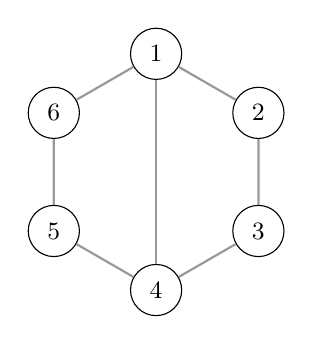
\begin{tikzpicture}
        \node[vtx, onslide=<2->{pick}] (v1) at (90:1.5)  {1};
        \node[vtx]                     (v2) at (30:1.5)  {2};
        \node[vtx, onslide=<2->{pick}] (v3) at (-30:1.5) {3};
        \node[vtx]                     (v4) at (-90:1.5) {4};
        \node[vtx, onslide=<2->{pick}] (v5) at (-150:1.5) {5};
        \node[vtx]                     (v6) at (150:1.5) {6};
        \draw[edg] (v1)--(v2)--(v3)--(v4)--(v5)--(v6)--(v1);
        \draw[edg] (v1)--(v4);
      \end{tikzpicture}
      \end{center}
    \end{column}
    \begin{column}{0.55\textwidth}
      \begin{itemize}
        \item<2-> $k = 3$: \alert{yes}. The set $\{1, 3, 5\}$ has no edge
              inside.
        \item<3-> $k = 4$: \alert{no}. Any $4$ of the $6$ vertices include two
              neighbors on the hexagon.
      \end{itemize}

      \medskip
      \onslide<3->{Same graph, different $k$: a different answer. The
      \emph{instance} is the pair $(G, k)$.}
    \end{column}
  \end{columns}
\end{frame}

\begin{frame}{Example: Subset Sum}
  $S = \{5, 8, 13, 4\}$. Does some subset sum to exactly $t$?

  \bigskip
  \begin{center}
  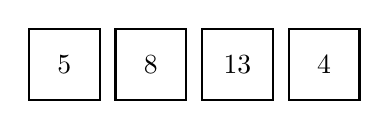
\begin{tikzpicture}[sq/.style={draw, thick, minimum size=9mm}]
    \node[sq] at (1.1,0) {5};
    \node[sq] at (2.2,0) {8};
    \node[sq, onslide=<2->{fill=mOrange!55}] at (3.3,0) {13};
    \node[sq, onslide=<2->{fill=mOrange!55}] at (4.4,0) {4};
  \end{tikzpicture}
  \end{center}

  \bigskip
  \begin{itemize}
    \item<2-> $t = 17$: \alert{yes}, since $13 + 4 = 17$.
    \item<3-> $t = 11$: \alert{no}. The $15$ nonempty subsets give the sums
          $4, 5, 8, 9, 12, 13, 17, 18, 21, 22, 25, 26, 30$, and $11$ is not
          among them.
  \end{itemize}

  \onslide<3->{\medskip To answer no, we checked every subset. With $n$
  numbers, that is $2^n$ of them.}
\end{frame}

\begin{frame}{Example: Graph Coloring}
  Can $G$ be colored with $\le k$ colors so that every edge has two different
  colors?

  \begin{columns}[c]
    \begin{column}{0.4\textwidth}
      \begin{center}
      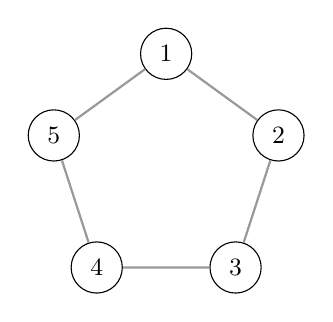
\begin{tikzpicture}
        \node[vtx, onslide=<3->{cA}] (v1) at (90:1.5)   {1};
        \node[vtx, onslide=<3->{cB}] (v2) at (18:1.5)   {2};
        \node[vtx, onslide=<3->{cA}] (v3) at (-54:1.5)  {3};
        \node[vtx, onslide=<3->{cB}] (v4) at (-126:1.5) {4};
        \node[vtx, onslide=<3->{cC}] (v5) at (162:1.5)  {5};
        \draw[edg] (v1)--(v2)--(v3)--(v4)--(v5)--(v1);
      \end{tikzpicture}
      \end{center}
    \end{column}
    \begin{column}{0.55\textwidth}
      \begin{itemize}
        \item<2-> $k = 2$: \alert{no}. Colors must alternate around the
              cycle, but it has odd length $5$, so vertices $5$ and $1$ would
              clash.
        \item<3-> $k = 3$: \alert{yes}. Alternate two colors and give
              vertex $5$ a third.
      \end{itemize}
    \end{column}
  \end{columns}
\end{frame}

% =========================================================================
\section{From Optimization to Decision}

\begin{frame}{Turning Optimization into Decision}
  Add a threshold $k$ to the objective. \alert{Minimize} becomes ``is there a
  solution of cost $\le k$?''; \alert{maximize} becomes ``is there one of
  value $\ge k$?''.

  \medskip
  \begin{center}
  \small
  \begin{tabular}{ll}
    \toprule
    optimization & decision \\
    \midrule
    find a shortest $s$--$t$ path & is there an $s$--$t$ path of length
      $\le k$? \\
    find a minimum spanning tree & is there a spanning tree of weight
      $\le k$? \\
    find a shortest tour of all cities & is there a tour of length
      $\le k$? \\
    find a largest independent set & is there an independent set of size
      $\ge k$? \\
    color $G$ with the fewest colors & can $G$ be colored with $\le k$
      colors? \\
    knapsack: most value within weight $W$ & is there a set of weight
      $\le W$ and value $\ge k$? \\
    \bottomrule
  \end{tabular}
  \end{center}
\end{frame}

\begin{frame}{Decision Is Just as Hard}
  \begin{itemize}
    \item The decision version is \alert{no harder}: solve the optimization
          problem, then compare the optimum with $k$.
    \item It is usually \alert{not easier} either: binary search over $k$
          recovers the optimal value.
  \end{itemize}

  \pause
  \bigskip
  \textbf{Example.} The fewest colors for $G$ is between $1$ and $n$.
  \begin{itemize}
    \item Ask ``$\le n/2$ colors?'', then halve the remaining range based on
          the answer.
    \item After $\lceil \log_2 n \rceil$ questions we know the exact minimum.
  \end{itemize}

  \medskip
  A fast algorithm for the decision version would give a fast algorithm for
  the optimization version. So it is enough to study \alert{decision}
  problems.
\end{frame}

% =========================================================================
\section{The Class P}

\begin{frame}{Polynomial Time and the Class P}
  An algorithm runs in \alert{polynomial time} if its worst-case running time
  is $O(n^c)$ for a constant $c$, where $n$ is the input size.

  \begin{block}{Definition}
    $\mathbf{P}$ is the class of decision problems that can be
    \alert{solved} in polynomial time.
  \end{block}

  \begin{itemize}
    \item \textbf{Shortest path} (no negative cycles): is there an
          $s$--$t$ path of length $\le k$? Dijkstra or Bellman-Ford.
    \item \textbf{Strongly connected components}: does $G$ have at most $k$
          SCCs? Two DFS passes, $O(n + m)$.
    \item \textbf{Minimum spanning tree}: is there a spanning tree of weight
          $\le k$? Prim or Kruskal.
  \end{itemize}
\end{frame}

\begin{frame}{Why Polynomial?}
  \begin{center}
  \begin{tabular}{rrrr}
    \toprule
    $n$ & $n^2$ & $n^3$ & $2^n$ \\
    \midrule
    10  & 100    & 1{,}000     & 1{,}024 \\
    50  & 2{,}500 & 125{,}000  & $1.1 \times 10^{15}$ \\
    100 & 10{,}000 & $10^6$    & $1.3 \times 10^{30}$ \\
    \bottomrule
  \end{tabular}
  \end{center}

  \bigskip
  \begin{itemize}
    \item At $10^9$ steps per second, $2^{100}$ steps take about
          $4 \times 10^{13}$ years.
    \item A faster computer barely helps an exponential algorithm: doubling
          the speed only adds $1$ to the $n$ we can handle.
    \item Polynomial is a coarse but robust notion of ``efficient'': it is
          closed under composition.
  \end{itemize}
\end{frame}

% =========================================================================
\section{Reductions}

\begin{frame}{Reductions}
  \begin{block}{Definition}
    $A$ \alert{polynomial-time reduces} to $B$, written $A \le_p B$, if there
    is a polynomial-time algorithm $f$ turning each instance $x$ of $A$ into
    an instance $f(x)$ of $B$ such that
    \[
      x \text{ is a yes-instance of } A \iff f(x) \text{ is a yes-instance of
      } B.
    \]
  \end{block}

  \begin{center}
  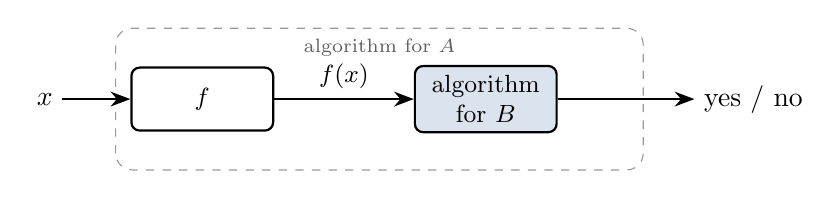
\begin{tikzpicture}
    \draw[dashed, mGray!80!black, rounded corners=6pt] (0.9,-0.9) rectangle (7.6,0.9);
    \node[font=\scriptsize, mGray!50!black] at (4.25,0.65) {algorithm for $A$};
    \node (x) at (0,0) {$x$};
    \node[box] (f) at (2,0) {$f$};
    \node[box, fill=mLightBlue!20] (b) at (5.6,0) {algorithm\\for $B$};
    \node (out) at (9,0) {yes / no};
    \draw[arr] (x) -- (f);
    \draw[arr] (f) -- node[above, font=\small] {$f(x)$} (b);
    \draw[arr] (b) -- (out);
  \end{tikzpicture}
  \end{center}

  Translate the question, then ask the $B$-solver. The answer is preserved.
\end{frame}

\begin{frame}{Example: Scheduling $\le_p$ Graph Coloring}
  \textbf{Scheduling}: $n$ tasks, $k$ time slots, and a list of conflicting
  pairs. Can every task get a slot so that conflicting tasks differ?

  \begin{columns}[c]
    \begin{column}{0.35\textwidth}
      \small
      Tasks $t_1, t_2, t_3, t_4$\\[2pt]
      Conflicts: $\{t_1, t_2\}$, $\{t_1, t_3\}$,\\
      \hphantom{Conflicts: }$\{t_2, t_3\}$, $\{t_3, t_4\}$\\[2pt]
      $k = 3$ slots
    \end{column}
    \begin{column}{0.12\textwidth}
      \begin{center}
      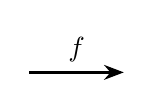
\begin{tikzpicture}
        \draw[arr, very thick] (0,0) -- node[above] {$f$} (1.2,0);
      \end{tikzpicture}
      \end{center}
    \end{column}
    \begin{column}{0.45\textwidth}
      \begin{center}
      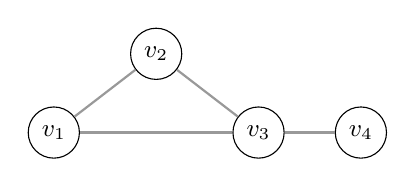
\begin{tikzpicture}
        \node[vtx, onslide=<2->{cA}] (1) at (0,0)    {$v_1$};
        \node[vtx, onslide=<2->{cB}] (2) at (1.3,1)  {$v_2$};
        \node[vtx, onslide=<2->{cC}] (3) at (2.6,0)  {$v_3$};
        \node[vtx, onslide=<2->{cA}] (4) at (3.9,0)  {$v_4$};
        \draw[edg] (1)--(2); \draw[edg] (1)--(3); \draw[edg] (2)--(3);
        \draw[edg] (3)--(4);
      \end{tikzpicture}
      \end{center}
    \end{column}
  \end{columns}

  \medskip
  \begin{itemize}
    \item One vertex per task, one edge per conflicting pair, same $k$.
          Time $O(n^2)$.
    \item<2-> Slot $=$ color: a schedule with $k$ slots is exactly a proper
          $k$-coloring, in both directions.
  \end{itemize}
\end{frame}

\begin{frame}{Reductions Transfer Algorithms}
  \begin{block}{Claim}
    If $A \le_p B$ and $B \in \mathbf{P}$, then $A \in \mathbf{P}$.
  \end{block}

  \textbf{Proof.} On input $x$ of size $n$:
  \begin{enumerate}
    \item Compute $f(x)$: time $O(n^c)$, so $|f(x)| = O(n^c)$ too (it cannot
          write more than it has time for).
    \item Run $B$'s algorithm on $f(x)$: time $O(|f(x)|^d) = O(n^{cd})$.
  \end{enumerate}
  Total time is polynomial, and the answer is correct by the definition of
  a reduction. \hfill $\square$

  \pause
  \bigskip
  \begin{block}{Contrapositive: hardness flows forward}
    If $A \le_p B$ and $A$ has no polynomial-time algorithm, then neither
    does $B$.
  \end{block}
  To show $B$ is hard, reduce \alert{from} a known hard problem \alert{to}
  $B$.
\end{frame}

% =========================================================================
\section{The Class NP}

\begin{frame}{Solving vs.\ Verifying}
  We know no polynomial-time algorithm for 3-coloring. But if someone hands
  us a coloring, \alert{checking} it is easy: look at every edge.

  \begin{columns}[c]
    \begin{column}{0.4\textwidth}
      \begin{center}
      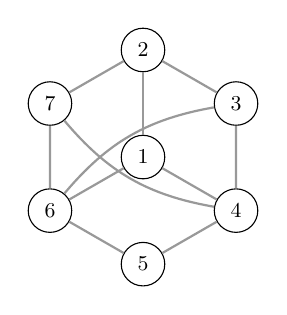
\begin{tikzpicture}[scale=0.85, every node/.append style={transform shape}]
        \sevengraph{vtx}{vtx}{vtx}{vtx}{vtx}{vtx}{vtx}
      \end{tikzpicture}\\[2pt]
      \small Is it 3-colorable?
      \end{center}
    \end{column}
    \begin{column}{0.15\textwidth}
      \begin{center}
      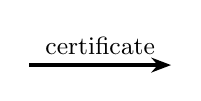
\begin{tikzpicture}
        \draw[arr, very thick] (0,0) -- node[above, font=\small] {certificate}
          (1.8,0);
      \end{tikzpicture}
      \end{center}
    \end{column}
    \begin{column}{0.4\textwidth}
      \begin{center}
      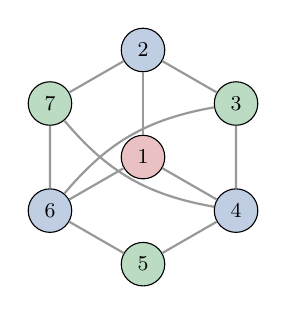
\begin{tikzpicture}[scale=0.85, every node/.append style={transform shape}]
        \sevengraph{cA}{cB}{cC}{cB}{cC}{cB}{cC}
      \end{tikzpicture}\\[2pt]
      \small Every edge has two colors: yes.
      \end{center}
    \end{column}
  \end{columns}
\end{frame}

\begin{frame}{The Class NP}
  \begin{block}{Definition}
    $\mathbf{NP}$ is the class of decision problems where every
    yes-instance has a \alert{certificate} (a short proof) that can be
    \alert{verified} in polynomial time.
  \end{block}

  \bigskip
  Think of a game between Alice and Bob.
  \begin{itemize}
    \item Alice knows the answer is yes and wants to convince Bob.
    \item Bob only runs polynomial-time algorithms, so he cannot search for
          a solution himself.
    \item Alice sends a certificate; Bob checks it.
  \end{itemize}

  \medskip
  No-instances need no certificate: whatever Alice sends, Bob must not be
  fooled.

  \pause
  \medskip
  \small NP stands for \emph{nondeterministic polynomial time}, not ``not
  polynomial''.
\end{frame}

\begin{frame}{Example: Independent Set $\in$ NP}
  An \alert{independent set} is a set $S$ of vertices with no edge inside.
  Given $G$ and $k$: is there one with $|S| \ge k$?

  \begin{columns}[c]
    \begin{column}{0.5\textwidth}
      \begin{center}
      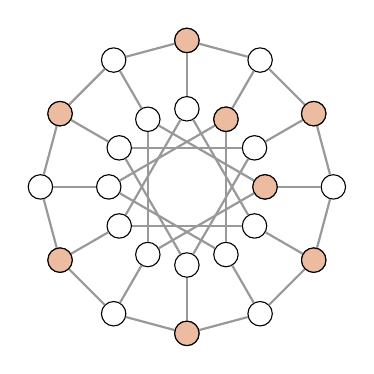
\begin{tikzpicture}[scale=0.62, every node/.append style={transform shape}]
        \foreach \i in {0,...,11} {
          \pgfmathsetmacro{\ang}{90 - \i * 30}
          \node[vtx, minimum size=5mm] (u\i) at (\ang:3)   {};
          \node[vtx, minimum size=5mm] (w\i) at (\ang:1.6) {};
        }
        \foreach \i [evaluate=\i as \j using {int(mod(\i+1,12))}] in {0,...,11}
          { \draw[edg] (u\i)--(u\j); }
        \foreach \i in {0,...,11} { \draw[edg] (u\i)--(w\i); }
        \foreach \i [evaluate=\i as \j using {int(mod(\i+4,12))}] in {0,...,11}
          { \draw[edg] (w\i)--(w\j); }
        \onslide<2->{
          \foreach \i in {0,2,4,6,8,10} { \node[pick, minimum size=5mm] at (u\i) {}; }
          \node[pick, minimum size=5mm] at (w1) {};
          \node[pick, minimum size=5mm] at (w3) {};
        }
      \end{tikzpicture}
      \end{center}
    \end{column}
    \begin{column}{0.45\textwidth}
      Is there an independent set of size $8$? Not obvious.

      \medskip
      \onslide<2->{\textbf{Certificate}: the set $S$ itself (orange).

      \medskip
      \textbf{Verify}: $|S| \ge 8$, and no edge has both ends in $S$.
      Time $O(n + m)$.}
    \end{column}
  \end{columns}
\end{frame}

\begin{frame}{Example: Subset Sum $\in$ NP}
  Given $S = \{3, 1, 7, 11, 4, 9, 2, 6\}$ and $t = 20$: does some subset sum
  to $20$?

  \bigskip
  \begin{center}
  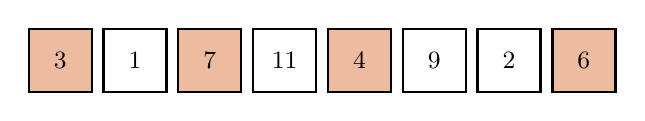
\begin{tikzpicture}[sq/.style={draw, thick, minimum size=8mm, font=\small}]
    \foreach \v [count=\i] in {3,1,7,11,4,9,2,6} {
      \node[sq] (s\i) at (\i*0.95,0) {\v};
    }
    \onslide<2->{
      \foreach \i in {1,3,5,8} { \node[sq, fill=mOrange!55] at (s\i) {}; }
      \node[font=\small] at (s1) {3}; \node[font=\small] at (s3) {7};
      \node[font=\small] at (s5) {4}; \node[font=\small] at (s8) {6};
    }
  \end{tikzpicture}
  \end{center}

  \bigskip
  \begin{itemize}
    \item Trying all $2^n$ subsets is too slow in general.
    \item<2-> \textbf{Certificate}: the subset $\{3, 7, 4, 6\}$.
    \item<2-> \textbf{Verify}: $3 + 7 + 4 + 6 = 20 = t$. Time $O(n)$.
  \end{itemize}
\end{frame}

\begin{frame}{P $\subseteq$ NP}
  \begin{block}{Claim}
    $\mathbf{P} \subseteq \mathbf{NP}$.
  \end{block}

  \textbf{Proof.} Let $L \in \mathbf{P}$ with polynomial-time algorithm
  $\mathcal{A}$. Verifier: on input $x$ and any certificate $c$, ignore $c$
  and run $\mathcal{A}(x)$. It runs in polynomial time and accepts exactly
  the yes-instances. \hfill $\square$

  \pause
  \bigskip
  \begin{block}{The big open question}
    Is $\mathbf{P} = \mathbf{NP}$? Can every problem whose solutions are
    easy to \emph{check} also be \emph{solved} easily?
  \end{block}

  \medskip
  Most researchers believe $\mathbf{P} \ne \mathbf{NP}$. It is one of the
  Clay Millennium Prize Problems (\$1{,}000{,}000).
\end{frame}

% =========================================================================
\begin{frame}{Exercise}
  \begin{enumerate}
    \item Show that Hamiltonian Cycle is in NP: what is the certificate, and
          how is it checked?
    \item Someone shows $\text{3-Coloring} \le_p X$ and also finds a
          polynomial-time algorithm for $X$. What follows?
    \item Someone shows $X \le_p \text{Shortest Path}$. Does that say
          anything about how hard $X$ is?
    \item Is it clear that ``$G$ is \alert{not} 3-colorable'' is in NP?
  \end{enumerate}
\end{frame}

\begin{frame}{Solution}
  \small
  \begin{enumerate}
    \item Certificate: the cycle, as an ordering $v_1, \ldots, v_n$ of the
          vertices. Check that every vertex appears exactly once and that
          $\{v_i, v_{i+1}\}$ and $\{v_n, v_1\}$ are edges. Time $O(n + m)$.
    \item 3-Coloring $\in \mathbf{P}$ by the claim. 3-Coloring is known
          to be NP-complete (next lecture's term), so this would even give
          $\mathbf{P} = \mathbf{NP}$.
    \item Yes, an upper bound: $X \in \mathbf{P}$, because Shortest Path is
          in $\mathbf{P}$. It says nothing about $X$ being hard.
    \item No. A coloring proves colorability, but there is no known short
          proof that \emph{no} coloring exists. Such ``complement'' problems
          form the class co-NP.
  \end{enumerate}
\end{frame}

% =========================================================================
\begin{frame}{Summary}
  \begin{itemize}
    \item \textbf{Decision problems}: yes/no answers; optimization problems
          have decision versions of the same difficulty.
    \item $\mathbf{P}$: decision problems \alert{solvable} in polynomial
          time.
    \item $\mathbf{NP}$: decision problems whose yes-instances have
          certificates \alert{verifiable} in polynomial time.
    \item $A \le_p B$: a polynomial-time translation preserving the answer.
          Algorithms flow backwards ($B$ easy $\Rightarrow$ $A$ easy),
          hardness flows forwards ($A$ hard $\Rightarrow$ $B$ hard).
    \item $\mathbf{P} \subseteq \mathbf{NP}$; whether they are equal is open.
  \end{itemize}
\end{frame}

\end{document}
